% ------------------------------------------------------------------------
\mysection{Reduced order models for an advection-diffusion equation on an overlapping grid} \label{eq:romAD}

Consider solving the advection diffusion equation on some domain $\Omega$, 
\begin{alignat}{3}
  & T_t + (\av\cdot\grad) T = \kappa \Delta T  + f_b(\xv,t),   \qquad&& \text{for $\xv\in\Omega$} \label{eq:ADequation}\\
  & T(\xv,0)=T_0(\xv),   \qquad&& \text{for $\xv\in\Omega$},\\
  & \alpha T + \beta \partial_n T = g(\xv,t) \qquad&& \text{for $\xv\in\partial\Omega$}, 
\end{alignat}
with some body forcing $f_b(\xv,t)$. 
We will solve these equations on an overlapping grid, $\Gc =\{ G_g \}_{g=1}^{\Nc_g}$, consisting of $\Nc_g$ component
grids. On each component grid $G_g$ we define a discrete approximation, $T_\iv^{n}\approx T(\xv_\iv,t^n)$.

Given a reduced (POD) basis $\{ \phiv_i \}_{i=1}^K$, where $\phiv_i \in\Real^M$ are vectors
representing $T_\iv^n$ at all grid points on all grids (there being a total of $M$ grid points). 

We look for a reduced order solution of the form
\begin{align}
   T^K(\xv,t) &=  \sum_{j=1}^K q_j(t)\phiv_j(\xv)  + \sum_{m=1}^{N_p} g_m(t)T^p_m(\xv,t)   . \label{eq:romSolutionAD}
\end{align}
for some unknowns $\{ q_i(t) \}$, and where $T_m^p(\xv,t)$ are {\em particular functions}, chosen, for example, to satisfy the boundary conditions.

Substituting~\eqref{eq:romSolutionAD} into the advection-diffusion equation~\eqref{eq:ADequation} gives
\begin{align}
  & T^K_t + (\av\cdot\grad)T^K = \kappa \Delta T^K + f_b(\xv,t),  \label{eq:romEquationAD} 
\end{align}
or
\begin{align}
  & \sum_{j=1}^K \frac{d q_j}{dt} \phiv_j  + \sum_{j=1}^K q_j (\av\cdot\grad)\phiv_j 
             = \kappa \sum_{j=1}^K q_j \Delta \phiv_j ~~ + F_b(\xv,t),  \\
  &  F_b(\xv,t)   = f_b(\xv,t) 
        -  \sum_m \Big\{ \partial_t[ g_m(t)T^p_m(\xv,t)] + g_m(t) (\av\cdot\grad)T^p_m(\xv,t) - g_m(t)\kappa \Delta T^p_m(\xv,t) \Big\}.
\end{align}

These last equations implicitly define (an over-determined) system of ODEs for the unknowns $\{ q_i(t) \}$. 
We can use a Galerkin projection to define a set of $N$ ODE equations for the $N$ unknowns $q_i(t)$. 

Let $<\cdot,\cdot>$ denote some inner product on $\Real^M$. 
Different choices for the inner-product will be considered. 


Taking the inner product of $\phiv_i$ with~\eqref{eq:romEquationAD} (i.e. we project the equations onto the space
spanned by $\{ \phiv_i \}$) gives
\begin{align}
  &   \sum_{j=1}^K M_{ij} \frac{d q_j}{dt}  + \sum_j B_{ij} q_j  =  \sum_{j=1}^K K_{ij} q_j(t)  + f_i,  \label{eq:ROM_AD_I}
\end{align}
where 
\begin{align}
&   M_{ij} = <\phiv_i,\phiv_j>, \qquad
  B_{ij}  = <\phiv_i, (\av\cdot\grad)\phiv_j>, \qquad 
  K_{ij} = <\phiv_i,\kappa \Delta \phiv_j>, \\
&  f_i =  - <\phiv_i, F_b>
% &  f_i =  - <\phiv_i, \partial_t T^p(\xv,t) + (\av^p\cdot\grad) T^p - \kappa\Delta T^p > + <\phiv_i,f_b(\xv,t)> 
\end{align}
Equations~\ref{eq:ROM_AD_I} can be written as
\begin{align}
  &  M \frac{d\qv}{dt} + B \qv = K \qv + \fv . \label{eq:romEquationProjectedAD} 
\end{align}




% =======================================================================================
\mysubsection{Cgad: advection-diffusion of a pulse past a cylinder} \label{sec:advectionDiffusionPastACylinder}

In this example we solve an advection diffusion equation (Cgad) for a pulse moving past a cylinder.
The boundary conditions are Neumann (check me).

We save 200 snapshots over the time interval $[0,2]$ so that the snap shot time interval is $\dt_s=.01$

We consider two ways to form the projected equations: (1) A Galerkin projection using the standard inner product
and (2) a Galerkin projection using the integration weights in the inner product.

Here are the first 21 singular values:
\begin{verbatim}
 151.71704 108.46108 79.70319 57.30043 33.02741 19.41691 10.25015 9.04892
 5.27542 2.52297 1.30634 1.00365 0.48398 0.21195 0.08702 0.03895 0.02111 
 0.01361 0.00904 0.00629 0.00445
\end{verbatim}

Figure~\ref{fig:advectionDiffusionROMresultsIW} shows results using the weighted inner-product (WIP) projection.
Figure~\ref{fig:advectionDiffusionROMresults} shows results using the standard inner-product (SIP) projection.
The projected initial conditions are accurate to about 4e-3 and 2e-9 for 10 and 20 POD modes, for either SIP or WIP.
The WIP scheme has errors of about 2.e-3 (10 modes) and 9.6e-4 (20) modes at t=1.5. Question: is the accuracy of the 20 mode
solution being limited by the frequency of snapshots?

The SIP scheme has errors about .1 (10 modes) and .12 (20) modes at t=1.5.

The WIP scheme is clearly much better in this case - but WHY?. We note that when solving the same
problem on a square Cartesian grid there is little difference between WIP and SIP so that the either the
overlap or the curvilinear grid has made a difference.



\begin{figure}[hbt]
\newcommand{\figWidth}{5.5cm}
\newcommand{\trimfig}[2]{\trimPlot{#1}{#2}{0.1}{.0}{.11}{.02}}
\begin{center}
\begin{tikzpicture}[scale=1]
  \useasboundingbox (0,1.) rectangle (16.,11.0);  % set the bounding box (so we have less surrounding white space)
%
  \draw ( 0.00, 0.) node[anchor=south west,xshift=-4pt,yshift=+0pt] {\trimfig{\romFigures/cic4Pulset0p5}{\figWidth}};
  \draw ( 5.4 , 0.) node[anchor=south west,xshift=-4pt,yshift=+0pt] {\trimfig{\romFigures/cic4Pulset1p0}{\figWidth}};
  \draw (10.8 , 0.) node[anchor=south west,xshift=-4pt,yshift=+0pt] {\trimfig{\romFigures/cic4Pulset1p5}{\figWidth}};
%
  \draw ( 0.00,5.5) node[anchor=south west,xshift=-4pt,yshift=+0pt] {\trimfig{\romFigures/cic4Pulset0p0}{\figWidth}};
  \draw ( 5.4 ,5.5) node[anchor=south west,xshift=-4pt,yshift=+0pt] {\trimfig{\romFigures/cic4Pulset0p1}{\figWidth}};
  \draw (10.8 ,5.5) node[anchor=south west,xshift=-4pt,yshift=+0pt] {\trimfig{\romFigures/cic4Pulset0p2}{\figWidth}};
%
 % \draw (current bounding box.south west) rectangle (current bounding box.north east);
% grid:
%\draw[step=1cm,gray] (0,0) grid (16,10);
\end{tikzpicture}
\end{center}
  \caption{Advection diffusion of a pulse moving past a cylinder. Solution at various times.}
  \label{fig:advectionDiffusionPulseSolution}
\end{figure}



\begin{figure}[hbt]
\newcommand{\figWidth}{5.5cm}
\newcommand{\trimfig}[2]{\trimPlot{#1}{#2}{0.1}{.0}{.11}{.02}}
\begin{center}
\begin{tikzpicture}[scale=1]
  \useasboundingbox (0,1.) rectangle (16.,11.0);  % set the bounding box (so we have less surrounding white space)
%
  \draw ( 0.00, 0.) node[anchor=south west,xshift=-4pt,yshift=+0pt] {\trimfig{\romFigures/cicPulsePODvector0}{\figWidth}};
  \draw ( 5.4 , 0.) node[anchor=south west,xshift=-4pt,yshift=+0pt] {\trimfig{\romFigures/cicPulsePODvector1}{\figWidth}};
  \draw (10.8 , 0.) node[anchor=south west,xshift=-4pt,yshift=+0pt] {\trimfig{\romFigures/cicPulsePODvector2}{\figWidth}};
%
  \draw ( 0.00,5.5) node[anchor=south west,xshift=-4pt,yshift=+0pt] {\trimfig{\romFigures/cicPulsePODvector3}{\figWidth}};
  \draw ( 5.4 ,5.5) node[anchor=south west,xshift=-4pt,yshift=+0pt] {\trimfig{\romFigures/cicPulsePODvector4}{\figWidth}};
  \draw (10.8 ,5.5) node[anchor=south west,xshift=-4pt,yshift=+0pt] {\trimfig{\romFigures/cicPulsePODvector5}{\figWidth}};
%
 % \draw (current bounding box.south west) rectangle (current bounding box.north east);
% grid:
%\draw[step=1cm,gray] (0,0) grid (16,10);
\end{tikzpicture}
\end{center}
  \caption{Advection diffusion of a pulse moving past a cylinder: first few POD vectors.}
  \label{fig:advectionDiffusionPODvectors}
\end{figure}

% cicPulseROM10PODt0.pdf
\begin{figure}[hbt]
\newcommand{\figWidth}{5.5cm}
\newcommand{\trimfig}[2]{\trimPlot{#1}{#2}{0.09}{.0}{.11}{.02}}
\begin{center}
\begin{tikzpicture}[scale=1]
  \useasboundingbox (0,1.) rectangle (16.5,18.);  % set the bounding box (so we have less surrounding white space)
%
  \draw ( 0.00, 0.) node[anchor=south west,xshift=-4pt,yshift=+0pt] {\trimfig{\romFigures/cicPulseIWROM10PODt0p0}{\figWidth}};
  \draw ( 5.5 , 0.) node[anchor=south west,xshift=-4pt,yshift=+0pt] {\trimfig{\romFigures/cicPulseIWROMErr10PODt0p0}{\figWidth}};
  \draw (11.0 , 0.) node[anchor=south west,xshift=-4pt,yshift=+0pt] {\trimfig{\romFigures/cicPulseIWROMErr20PODt0p0}{\figWidth}};
%
  \draw ( 0.00,5.5) node[anchor=south west,xshift=-4pt,yshift=+0pt] {\trimfig{\romFigures/cicPulseIWROM10PODt0p5}{\figWidth}};
  \draw ( 5.5 ,5.5) node[anchor=south west,xshift=-4pt,yshift=+0pt] {\trimfig{\romFigures/cicPulseIWROMErr10PODt0p5}{\figWidth}};
  \draw (11.00,5.5) node[anchor=south west,xshift=-4pt,yshift=+0pt] {\trimfig{\romFigures/cicPulseIWROMErr20PODt0p5}{\figWidth}};
%
  \draw ( 0.00,11.0) node[anchor=south west,xshift=-4pt,yshift=+0pt] {\trimfig{\romFigures/cicPulseIWROM10PODt1p5}{\figWidth}};
  \draw ( 5.50,11.0) node[anchor=south west,xshift=-4pt,yshift=+0pt] {\trimfig{\romFigures/cicPulseIWROMErr10PODt1p5}{\figWidth}};
  \draw (11.00,11.0) node[anchor=south west,xshift=-4pt,yshift=+0pt] {\trimfig{\romFigures/cicPulseIWROMErr20PODt1p5}{\figWidth}};
%
 % \draw (current bounding box.south west) rectangle (current bounding box.north east);
% grid:
%\draw[step=1cm,gray] (0,0) grid (16,15);
\end{tikzpicture}
\end{center}
  \caption{WIP: advection diffusion of a pulse moving past a cylinder: Galerkin projection WITH weighted inner product. Left: solution computed
with 10 POD modes. Middle: error using 10 POD modes. Right: error using 20 POD modes.}
  \label{fig:advectionDiffusionROMresultsIW}
\end{figure}


\begin{figure}[hbt]
\newcommand{\figWidth}{5.5cm}
\newcommand{\trimfig}[2]{\trimPlot{#1}{#2}{0.09}{.0}{.11}{.02}}
\begin{center}
\begin{tikzpicture}[scale=1]
  \useasboundingbox (0,1.) rectangle (16.5,18.);  % set the bounding box (so we have less surrounding white space)
%
  \draw ( 0.00, 0.) node[anchor=south west,xshift=-4pt,yshift=+0pt] {\trimfig{\romFigures/cicPulseROM10PODt0p0}{\figWidth}};
  \draw ( 5.5 , 0.) node[anchor=south west,xshift=-4pt,yshift=+0pt] {\trimfig{\romFigures/cicPulseROMErr10PODt0p0}{\figWidth}};
  \draw (11.0 , 0.) node[anchor=south west,xshift=-4pt,yshift=+0pt] {\trimfig{\romFigures/cicPulseROMErr20PODt0p0}{\figWidth}};
%
  \draw ( 0.00,5.5) node[anchor=south west,xshift=-4pt,yshift=+0pt] {\trimfig{\romFigures/cicPulseROM10PODt0p5}{\figWidth}};
  \draw ( 5.5 ,5.5) node[anchor=south west,xshift=-4pt,yshift=+0pt] {\trimfig{\romFigures/cicPulseROMErr10PODt0p5}{\figWidth}};
  \draw (11.0 ,5.5) node[anchor=south west,xshift=-4pt,yshift=+0pt] {\trimfig{\romFigures/cicPulseROMErr20PODt0p5}{\figWidth}};
%
  \draw ( 0.00,11.0) node[anchor=south west,xshift=-4pt,yshift=+0pt] {\trimfig{\romFigures/cicPulseROM10PODt1p5}{\figWidth}};
  \draw ( 5.50,11.0) node[anchor=south west,xshift=-4pt,yshift=+0pt] {\trimfig{\romFigures/cicPulseROMErr10PODt1p5}{\figWidth}};
  \draw (11.00,11.0) node[anchor=south west,xshift=-4pt,yshift=+0pt] {\trimfig{\romFigures/cicPulseROMErr20PODt1p5}{\figWidth}};
%
 % \draw (current bounding box.south west) rectangle (current bounding box.north east);
% grid:
% \draw[step=1cm,gray] (0,0) grid (16,15);
\end{tikzpicture}
\end{center}
  \caption{SIP: advection diffusion of a pulse moving past a cylinder: Galerkin projection with NO weights in the inner product. Left: solution computed
with 10 POD modes. Middle: error using 10 POD modes. Right: error using 20 POD modes.}
  \label{fig:advectionDiffusionROMresults}
\end{figure}



% =======================================================================================
\clearpage
\mysubsection{Cgad: square with heated holes} \label{sec:CgadSquareWithHeatedHoles}


In this section we consider a problem with inhomogeneous and time varying boundary conditions.
Particular functions are used to satisfy the boundary conditions.

% makeAnnulus(.3,0,.4,annulus1);
% makeAnnulus(.2,-.4,-.4,annulus2);
% makeAnnulus(.2, .4,-.4,annulus3);
The geometry of the problem consists of a square domain $\Rc = [-1,1]^2$ with $N_c=3$ cylindrical holes, 
$\Cc_k=\{ \vert \xv - \cv_k \| < r_k \}$, with 
$\cv_1=(0,.4)$, $r_1=0.3$, 
$\cv_1=(-.4,-.4)$, $r_1=0.2$,  and 
$\cv_1=( .4,-.4)$, $r_1=0.2$.

\noindent{\bf Step 1 - particular boundary functions:} Create 3 particular functions, $\fv_k^p(\xv)$, 
for imposing the boundary conditions. The function $\fv_k^p$ is equal to the 
approximate steady state solution to the heat equation with $T=1$ on $\partial \Cc_k$ and $T=0$ on other boundaries.

{\scriptsize
\begin{verbatim}
cgad heatedSquareWithHoles -g=squareWithHolesGride8.order2 -T1=0. -T2=0. -T3=1. -ts=im -tp=.5 -tf=2. -show=heatedSquareWithHolesAnnulus3ParticularFunction.show -go=halt

cgad heatedSquareWithHoles -g=squareWithHolesGride8.order2 -T1=0. -T2=1. -T3=0. -ts=im -tp=.5 -tf=2. -show=heatedSquareWithHolesAnnulus2ParticularFunction.show -go=halt

cgad heatedSquareWithHoles -g=squareWithHolesGride8.order2 -T1=1. -T2=0. -T3=0. -ts=im -tp=.5 -tf=2. -show=heatedSquareWithHolesAnnulus1ParticularFunction.show -go=halt
\end{verbatim}
}

\noindent{\bf Step 2 - construct snapshots:} Create snapshots, $\sv^n\approx T(\xv,t^n)$, $n=1,2,\ldots,N$,
 by solving the heat equation with initial conditions $T_0(\xv)=$ and
boundary conditions $T_k^b(t) = \alpha_k t$, $k=1,2,3$, with $\alpha_1=1$, $\alpha_2=1$ and $\alpha_3=0$. 
We save snapshots at $t^n=n\Delta$, $\Delta=.05$ for $t\in[0,2]$. 
This solution will be denoted as $T^{\rm snap}$. 

{\scriptsize
\begin{verbatim}
cgad heatedSquareWithHoles -g=squareWithHolesGride4.order2 -T1a1=1. -T2a1=1. -ts=im -tp=.05 -tf=2. -show=heatedSquareWHRamp1and2.show -go=halt
\end{verbatim}
}


\noindent{\bf Step 3 - construct ROM:} Build a Galerkin ROM for the heat equation from a POD basis for the snapshots. 
The cardinality of the POD basis is $M$.


\noindent{\bf Step 4- evaluate ROM:} Solve the ROM for some different cases and compute the errors.
\begin{description}
  \item[Case 1:] Boundary conditions are $g_k(t) = \alpha_k t$, $k=1,2,3$, with $\alpha_1=1$, $\alpha_2=1$ and $\alpha_3=0$. These
    are the same conditions used to generate $T^{\rm snap}$.
  \item[Case 2:] 
  \item[Case 3:]
\end{description}


Figure~\ref{fig:CgadSquareWithHoles} shows the solution from a heat condition problem where the temperature
on the boundaries of two annulii is assigned to linearly increase over time. Two particular functions are
used to enforce the boundary conditions.

\begin{figure}[hbt]
\newcommand{\figWidth}{5.5cm}
\newcommand{\trimfig}[2]{\trimPlot{#1}{#2}{0.1}{.0}{.11}{.02}}
\begin{center}
\begin{tikzpicture}[scale=1]
  \useasboundingbox (0,1.) rectangle (16.,6.0);  % set the bounding box (so we have less surrounding white space)
%
  \draw ( 0.00, 0.) node[anchor=south west,xshift=-4pt,yshift=+0pt] {\trimfig{\romFigures/heatedSquareWithHolesA1A2ROM10_T_t1p0}{\figWidth}};
  \draw ( 5.4 , 0.) node[anchor=south west,xshift=-4pt,yshift=+0pt] {\trimfig{\romFigures/heatedSquareWithHolesA1A2ROM10_Terr_t1p0}{\figWidth}};
%  \draw (10.8 , 0.) node[anchor=south west,xshift=-4pt,yshift=+0pt] {\trimfig{\romFigures/cicPulsePODvector2}{\figWidth}};
%
%  \draw ( 0.00,5.5) node[anchor=south west,xshift=-4pt,yshift=+0pt] {\trimfig{\romFigures/cicPulsePODvector3}{\figWidth}};
%  \draw ( 5.4 ,5.5) node[anchor=south west,xshift=-4pt,yshift=+0pt] {\trimfig{\romFigures/cicPulsePODvector4}{\figWidth}};
%  \draw (10.8 ,5.5) node[anchor=south west,xshift=-4pt,yshift=+0pt] {\trimfig{\romFigures/cicPulsePODvector5}{\figWidth}};
%
 % \draw (current bounding box.south west) rectangle (current bounding box.north east);
% grid:
%\draw[step=1cm,gray] (0,0) grid (16,10);
\end{tikzpicture}
\end{center}
  \caption{A square with heated holes illustrating the use of particular functions to enforce the time varying boundary condtions.
   Left: solution at $t=1.$. Right: error at $t=1.$ using $K=10$ POD modes. Two PF's were used to assign the boundary conditions.
   }
  \label{fig:CgadSquareWithHoles}
\end{figure}


\begin{figure}[hbt]

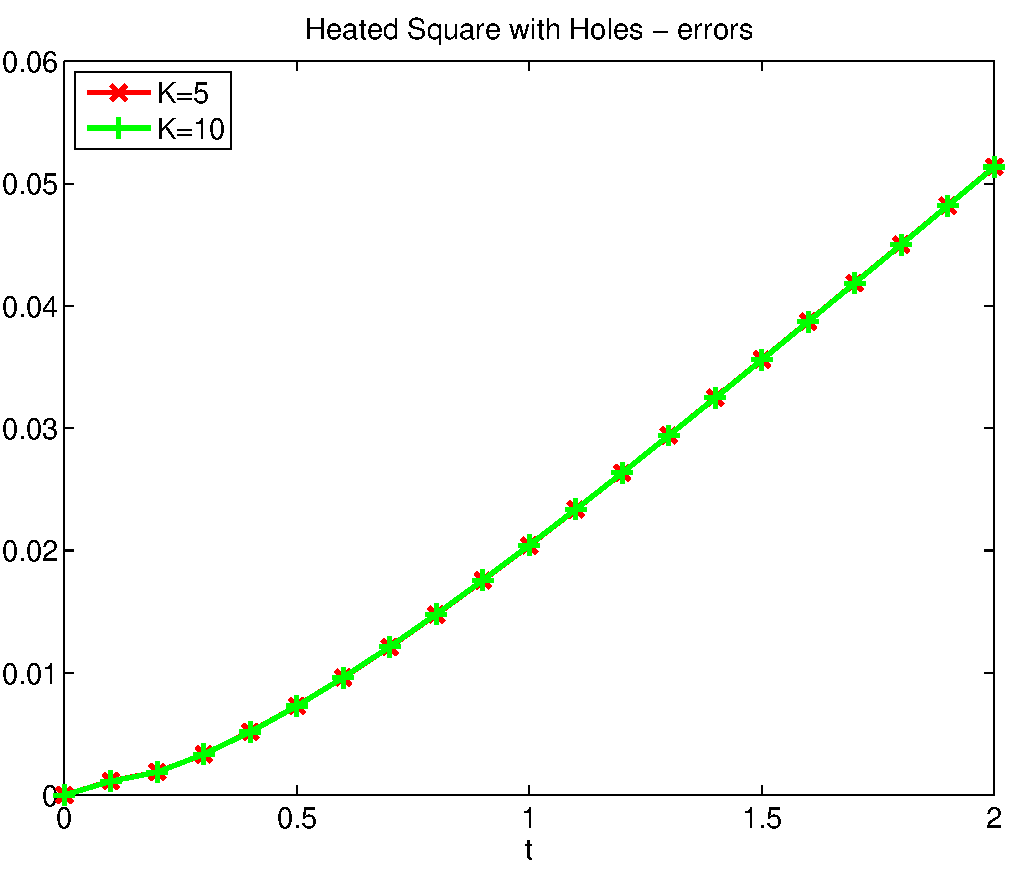
\includegraphics[width=8cm]{\romFigures/heatedSquareWithHolesRamp1And2Errors}

\caption{Errors for the square with heated holes ===FINISH ME===}

\end{figure}


\clearpage
Figure~\ref{fig:CgadSquareWith8Holes} shows the solution from a heat condition problem where the temperatures
on the boundaries of three annulii are assigned to linearly increase over time. Three particular functions are
used to enforce the boundary conditions.

\begin{figure}[hbt]
\newcommand{\figWidth}{7.5cm}
\newcommand{\trimfig}[2]{\trimPlot{#1}{#2}{0.1}{.0}{.11}{.02}}
\begin{center}
\begin{tikzpicture}[scale=1]
  \useasboundingbox (0,1.) rectangle (16.,14.);  % set the bounding box (so we have less surrounding white space)
%
  \draw ( 0.00,7.0) node[anchor=south west,xshift=-4pt,yshift=+0pt] {\trimfig{\romFigures/square8HolesRampA1A4A6_K10_Trom_0p2}{\figWidth}};
  \draw ( 7.4 ,7.0) node[anchor=south west,xshift=-4pt,yshift=+0pt] {\trimfig{\romFigures/square8HolesRampA1A4A6_K10_Terr_0p2}{\figWidth}};
%
  \draw ( 0.00, 0.) node[anchor=south west,xshift=-4pt,yshift=+0pt] {\trimfig{\romFigures/square8HolesRampA1A4A6_K10_Trom_1p0}{\figWidth}};
  \draw ( 7.4 , 0.) node[anchor=south west,xshift=-4pt,yshift=+0pt] {\trimfig{\romFigures/square8HolesRampA1A4A6_K10_Terr_1p0}{\figWidth}};
%
 % \draw (current bounding box.south west) rectangle (current bounding box.north east);
% grid:
% \draw[step=1cm,gray] (0,0) grid (15,15);
\end{tikzpicture}
\end{center}
  \caption{A square with heated holes illustrating the use of particular functions to enforce the time varying boundary condtions.
   Top: solution and error at $t=.2$. Bottom: solution and error at $t=1.$. $K=10$ POD modes were used. Three PF's were used to assign the boundary conditions.
   }
  \label{fig:CgadSquareWith8Holes}
\end{figure}




\begin{figure}[hbt]
\newcommand{\figWidth}{5.5cm}
\newcommand{\trimfig}[2]{\trimPlot{#1}{#2}{0.1}{.0}{.11}{.02}}
\begin{center}
\begin{tikzpicture}[scale=1]
  \useasboundingbox (0,1.) rectangle (16.,5.2);  % set the bounding box (so we have less surrounding white space)
%
  \draw ( 0.00, 0.) node[anchor=south west,xshift=-4pt,yshift=+0pt] {\trimfig{\romFigures/square8HolesRampA1A4A6_PF1}{\figWidth}};
  \draw ( 5.4 , 0.) node[anchor=south west,xshift=-4pt,yshift=+0pt] {\trimfig{\romFigures/square8HolesRampA1A4A6_PF2}{\figWidth}};
  \draw (10.8 , 0.) node[anchor=south west,xshift=-4pt,yshift=+0pt] {\trimfig{\romFigures/square8HolesRampA1A4A6_PF3}{\figWidth}};
% grid:
% \draw[step=1cm,gray] (0,0) grid (16,5);
\end{tikzpicture}
\end{center}
  \caption{Particular functions used to assign the boundary conditions.}
  \label{fig:CgadSquareWith8HolesParticularFunctions}
\end{figure}


